\documentclass[psfig,preprint]{aastex}

\makeatletter
\renewcommand\theequation{\thesection.\arabic{equation}}
	\@addtoreset{equation}{section}
\renewcommand\thefigure{\thesection.\arabic{figure}}
	\@addtoreset{figure}{section}
\renewcommand\thetable{\thetable.\arabic{table}}
	\@addtoreset{table}{section}
\makeatother

\begin{document}

\setcounter{section}{-1}

\title{LEAST-SQUARES LITE FOR THE BUDDING AFICIONADO: \\ 
ART AND PRACTICE } 

\author{\copyright Carl Heiles and Deepthi Gorthi\footnote{Translation from IDL to Python}\\ \today }

	In our never-ending attempt to make your life easier, we present
you with this highly instructive, time-saving, and labor-saving
informative document! Here we give heuristic derivations, discussions,
examples, and the prescription for doing least-squares the easy way
using matrix techniques generally, and specifically in Python.  This
prescription is given as an example in \S\ref{numexample}, and the {\it
power-user} can skip the details and go directly there.  

	This document contains selected sections from the more complete
{\it LEAST-SQUARES AND CHI-SQUARE FOR THE BUDDING AFICIONADO: ART AND
PRACTICE}, which also covers advanced topics including covariance in
chi-square fitting, singular value decomposition, median and Minimum
Weighted Absolute Residuals Sum (MWARS) fitting, and fitting when both
$x$ and $y$ have uncertainties.  The full document runs to 62 pages,
which is a little intimidating for the novice.  We occasionally refer to
the books Bevington and Robinson (1992; BR), Cowan (1998), Press et al.\
(2001; Numerical Recipes, NR) and Taylor (1997; T97), and we update the
notation to partially conform with NR. 

	We begin with least-squares in the classic sense, meaning we
minimize the sum of squares instead of minimizing $\chi^2$\footnote{The $\chi^2$
is the sum of squares down-weighted by uncertainity in the measurement. Roughly 
because, poor measurements should influence the outcome to a smaller extent}. In
astronomy,  more often than not you don't have an independent assessment
of the intrinsic uncertainty in the data, which means you cannot
evaluate $\chi^2$, and the least squares  approach is the only option.
However, often in astronomy you do want to weight observations
differently, e.g.\ because of integration time, and this requires an
approach similar to the $\chi^2$ one. In later sections we generalize to
the $\chi^2$ and this other weighted-observations case.

\tableofcontents

\section{LEAST-SQUARES FITTING FOR TWO PARAMETERS, AS WITH A STRAIGHT
LINE.} \label{sectionone}

\subsection{The closed-form expressions for a straight-line fit}

	First consider the least-squares fit to a straight line.  Let
$y_m$ be the $m^{th}$ measurement of the observed quantity (in this
example, $y_m$ is distance; $t_m$ be the time of the
$m^{th}$ measurement; $M$ = the total number of observations, i.e.\ $m$
runs from 0 to $M-1$.  Remember that in the least-squares technique,
quantities such as $t_m$ are regarded to be known with high accuracy
while the quantity $y_m$ has uncertainties in its measurement. 

	We expect distance $y_m$ to change linearly with
time as follows:

\begin{equation} \label{one}
A + B t_m = y_m
\end{equation}

\noindent Given this, one does the maximum likelihood (ML) estimate assuming
Gaussian statistics. When all measurements have the same intrinsic
uncertainty, this is the same as looking for the solution that minimizes
the sum of the squares of the residuals (which we will define later). 
This leads to the pair of equations (Taylor 8.8, 8.9), called the {\it
normal equations}

\begin{mathletters} \label{normalone}
\begin{equation}
AN + B \ \sum t_m = \sum y_m
\end{equation}
\begin{equation}
A \ \sum t_m + B \ \sum t_m^2 = \sum t_m y_m \ .
\end{equation}
\end{mathletters}

\noindent Two equations and two unknowns---easy to solve! The
closed-form equations for $(A,B)$ are Taylor's equations 8.10 to 8.12.

\subsection{Better is the following generalized notation.}

	We want a way to generalize this approach to include any
functional dependence on $t$ and even other variables, and to have an
arbitrarily large number of unknown coefficients instead of just the two
$(A,B)$. This is very easy using matrix math.  We will ease into this
matrix technique gently, by first  carrying through an intermediate
stage of notation. 

	First generalize the straight-line fit slightly by having two
functional dependences instead of one. We have something other than the
time $t_m$; call it $s_m$. For example, we could have $s_m = \cos (t_m)$
or $s_m = t_m^2$; or we could have $s_m = x_m$, where $x_m$ is the
position from which the observation was taken. To correspond to equation
\ref{one}, $s_m = 1$. Then we rewrite equation \ref{one} to include this
extra dependence

\begin{equation} \label{two}
A s_m + B t_m = y_m \; .
\end{equation}

\noindent There are still only two unknown parameters, so this is an
almost trivial generalization; later we'll generalize to more
parameters.

	We have $M$ equations like equation \ref{two}, one for each
measurement.  They are known as the {\it equations of condition} because
they are the equations that specify the theoretical model to which we
are fitting the data. There are $M$ equations of condition and only two
unknowns ($A$ and $B$).  This is too many equations! We have to end up
with a system in which the number of equations is equal to the number of
unknowns.

	To accomplish this, from equation \ref{two} we form the {\it
normal equations}.  The number of normal equations is equal to the
number of unknowns, so in this case we will have two.   We could carry
through the same ML derivation to derive equations equivalent to
equation \ref{normalone}; the result is

\begin{mathletters} \label{ones}
\begin{equation}
A\ \sum s_m^2 + B \ \sum s_m t_m = \sum s_m y_m
\end{equation}
\begin{equation}
A \ \sum s_m t_m + B \ \sum t_m^2  = \sum t_m y_m \ .
\end{equation}
\end{mathletters}

\noindent We can rewrite these equations using the notation $[st] =
\sum s_m t_m$, etc.:

\begin{mathletters} \label{normaltwo}
\begin{equation}
A [ s^2 ] + B [ s t ] = [ s y ]
\end{equation}
\begin{equation}
A [ s t ] + B [ t^2 ] = [ t y ] \ .
\end{equation}
\end{mathletters}

\noindent This is, of course, precisely analogous to equation
\ref{normalone}. And now it's clear how to generalize to more
parameters!

\section{LEAST-SQUARES FITTING FOR MANY PARAMETERS, AS WITH A CUBIC}
\label{sectiontwo}

	With this notation it's easy to generalize to more ($N$)
unknowns: the method is obvious because in each equation of condition
(like equation \ref{two}) we simply add equivalent additional terms such
as $C u_m$, $D v_m$, etc; and in the normal equations (equation
\ref{normaltwo}) we have more products and also more normal equations. 

	Let's take an example with four unknowns ($N=4$), which we will
denote by $A, B, C, D$; this would be like fitting a cubic.  With $N=4$
we need at least five datapoints ($M=5$), so there must be at least
five equations of condition.  The generalization of equation \ref{ones}
is the $M$ equations

\begin{equation} \label{eqcond}
A s_m + B t_m + C u_m + D v_m = y_m \; ,
\end{equation}

\noindent with $m = 0 \rightarrow (M-1)$.  Again, the
least-squares-fitting process assumes that the $s_m, t_m, u_m, v_m$ are
known with zero uncertainty; all of the uncertainties are in the
measurements of $y_m$.  We then form the four normal equations; the
generalization of equation \ref{normaltwo} written in matrix format is:

\begin{eqnarray} \label{smeqn} 
\left[ 
\begin{array}{cccc} 
{[ ss ]} & {[ st ]} & {[ su ]} & {[ sv ]} \\ 
{[ ts ]} & {[ tt ]} & {[ tu ]} & {[ tv ]} \\ 
{[ us ]} & {[ ut ]} & {[ uu ]} & {[ uv ]} \\ 
{[ vs ]} & {[ vt ]} & {[ vu ]} & {[ vv ]} \\
\end{array} 
\; \right] 
\left[ 
\begin{array}{c} 
A \\ 
B \\ 
C \\ 
D \\
\end{array} 
\; \right] 
\; = 
\left[ 
\begin{array}{c} 
{[ s y ]} \\ 
{[ t y ]} \\ 
{[ u y ]} \\ 
{[ v y ]} \\ 
\end{array} 
\; \right]
\end{eqnarray} 

\noindent The $N \times N$ matrix on the left is symmetric. With $N$
equations and $N$ unknowns, you can actually {\it solve} for $A, B, C,
D$! 

\section{FAR, FAR BEST AND EASIEST: MATRIX ALGEBRA} \label{matrixmethod}

	The above equations are terribly cumbersome to solve in a
computer code because they require lots of loops.  However, it becomes
trivial if we use matrices.  Here we designate a {\bf matrix} by {\bf
boldface} type. 

	We illustrate the matrix method by carrying through the above
$N=4$ example, and we assume that there are 5 independent measurements
($M=5$).  We first define the matrices

\begin{mathletters} \label{matrixdefinition}
\begin{eqnarray} 
{\bf X} = \left[
\begin{array}{cccc} 
{s_0} & {t_0} & {u_0} & {v_0} \\ 
{s_1} & {t_1} & {u_1} & {v_1} \\ 
{s_2} & {t_2} & {u_2} & {v_2} \\ 
{s_3} & {t_3} & {u_3} & {v_3} \\
{s_4} & {t_4} & {u_4} & {v_4} \\
\end{array} 
\; \right] 
\end{eqnarray}
%\end{mathletters}

%\begin{mathletters}
\begin{eqnarray}
{\bf a} = \left[
\begin{array}{c}
A \\
B \\
C \\
D \\
\end{array} \; \right] 
\end{eqnarray}
%\end{mathletters}

%\begin{mathletters}
\begin{eqnarray}
{\bf Y} = \left[
\begin{array}{c} 
{y_0} \\ 
{y_1} \\ 
{y_2} \\ 
{y_3} \\ 
{y_4} \\ 
\end{array} 
\; \right]
\end{eqnarray} 
\end{mathletters} 

\noindent so, in matrix form, the equations of condition (equation
\ref{eqcond}) reduce to the single matrix equation

\begin{equation}
\label{equationofcondition}
{\bf X \cdot a} = {\bf Y} \; .
\end{equation}

\noindent The notation for these equations corresponds to NR's. We write
them with subscripts $\sigma$ to emphasize that they are calculated
without dividing by $\sigma_{meas}$, i.e.\ that we are doing least
squares instead of chi-square fitting. For chi-square fitting, see \S
\ref{chisqsection} and \ref{chicoeffsnoco}.

	Our matrix $\mathbf{X}$ corresponds to NR's ``design
matrix'' $\bf A$ of Figure 15.4.1, except that our elements are not
divided by $\sigma_{meas,m}$, and the matrix equation of condition
(equation \ref{equationofcondition}) is identical to the expression
inside the square brackets of NR's equation 15.4.6. The differences
arise because here we are discussing least-squares fitting instead of
chi-square fitting, i.e.\ we have omitted the factors involving
$\sigma_{meas,m}$, the intrinsic measurement uncertainties (\S
\ref{chisqsection}).

	Again, there are more equations than unknowns so we can't solve
this matrix equation directly.  So next we form the normal equations
from these matrices.  In matrix form, the normal equations (equation
\ref{smeqn}) reduce to the single equation 

\begin{equation} \label{matrixnormal}
\mathbf{[\alpha] \cdot a} = \mathbf{[\beta]} \; ,
\end{equation}

\noindent (NR equation 15.4.10), where

\begin{mathletters} 
\label{ssdef}
\begin{equation} 
[\alpha] = {\bf X^T \cdot X} 
\end{equation}
\begin{equation}
[\beta] = {\bf X^T \cdot Y} \ .
\end{equation}
\end{mathletters}

\noindent The matrix $[\alpha]$ is known as the {\it curvature
matrix} because each element is twice the curvature of $\sigma^2$ (or
$\chi^2$) plotted against the corresponding product of variables. 

	The number of equations is equal to the number of unknowns, so
the solution of the matrix equation is easy---just rewrite it by
multiplying both sides by the inverse of $[\alpha]$ (that is, by
$[\alpha]^{-1})$, which gives

\begin{equation}
\label{adef}
{\bf a} = [\alpha]^{-1} \mathbf{ \cdot [\beta]} \; .
\end{equation}

\noindent All of these matrix operations are trivially easy in Python (\S
\ref{numexample}). 

\section{UNCERTAINTIES IN THE DERIVED COEFFICIENTS} \label{sigmas}

	How about the uncertainties in the derived quantities contained
in the matrix ${\bf a}$?

       The first thing to do is derive the {\it sample} variance $s^2$
(the square of standard deviation, or mean error, or dispersion, etc) of
the individual datapoints using the generalization of the usual
definition for a straight average of $x$, $s^2 = [ \sum_0^{M-1} (x_m -
\overline{ x_m})^2/(M-1)]$.  The generalization is, simply, to replace   
the $M-1$ in the denominator by $\nu = M-N$.  In the straight-average
case, $N=1$ so this fits. Here $\nu$ is known as the number of {\it
degrees of freedom} and $N$, the number of unknown coefficients, is
known as the number of {\it constraints}. So we have

\begin{equation} \label{samplevarianceone}
s^2 = {1 \over M - N} \sum_{m=0}^{M-1} (y_m -
\overline{y_m})^2 \; ,
\end{equation}  

\noindent where $\overline{y_m}$ are the values for $y_m$ {\it
predicted by the derived quantities ${\bf a}$}. Note the difference:
$y_m$ are the {\it observed} values, while $\overline{y_m}$ are the
values {\it predicted by the least-squares fit}.  The predicted values
are those that are computed from the derived coefficients $A, B, C$\dots
The $M$ quantities

\begin{equation} \label{sequation}
\delta y_m = y_m - \overline{y_m}
\end{equation}

\noindent are called the {\it residuals} or {\it deviations} from the
fit.

        It's worth reiterating some essentials about $s^2$, and in
particular the denominator $(M-N)$.  First consider the case of a
single-parameter fit, e.g.\ $N=1$.  Then we cannot possibly derive a
sample variance from only one measurement $M=1$; but we can from two
$M=2$.  So the denominator makes sense from that standpoint.  The same
goes for $N>1$. 

        Next consider the effect of using $(M-N)$ in the denominator: it
increases $s^2$ by the ratio ${M \over M-N}$ over what you'd get if you
just took a straight average and used $M$. This compensates for the fact
that you are subtracting $\overline {y_m}$, which is derived from
the data, instead of the {\it truly} correct value $y^*$. (In
formal statistical language, $y^*$ is the mean of the parent
population from which your set of measurements is drawn.) If you used
the truly correct value $y^*$, then the sum would be larger than
when using $\overline{ y_m}$. The use of $M-N$ in the denominator
compensates for this larger value in exactly the right way: the
expectation value $E_{(s^2)}$ for a large number of experiments is
precisely equal to the normal variance $\sigma^2$, which you'd get by
using [$y^*$ and $M$] instead of [$\overline{y_m}$ and
$(M-N)$] in equation \ref{sequation}; see Cowan equations 5.9 and 5.10.
So $s^2$ is, in fact, exactly the number  we want: an unbiased estimate
of the true variance of our sample. Why    not use [$y^*$ and $M$]
in equation \ref{sequation}? The reason is obvious: we don't know
$y^*$! (If we did, we wouldn't be doing this analysis!)

	It's easy to calculate the $\overline{y_m}$ with matrices.
First define the matrix ${\bf \overline{ Y}}$ that contains these
values:

\begin{eqnarray}
{\bf \overline{ Y}} = \left[
\begin{array}{c} 
\overline{y_0} \\ 
\overline{y_1} \\ 
\overline{y_2} \\ 
\overline{y_3} \\ 
\overline{y_4} \\ 
\end{array} 
\; \right]
\end{eqnarray} 

{\noindent} Calculating ${\bf \overline{ Y}}$ is simple:

\begin{equation} \label{ybardefinition}
{\bf \overline{ Y}} = {\bf  X \cdot a} \; . 
\end{equation}

\noindent Note that ${\bf X}$ is already defined (equation
\ref{matrixdefinition}) and ${\bf a}$ was solved for in equation
\ref{adef}. It's convenient to define the residual matrix

\begin{equation}
{\bf \delta Y } = {\bf Y - \overline{ Y}}
\end{equation}

\noindent so we can write

\begin{equation} \label{samplevariancetwo}
s^2 = {1 \over M - N} {\bf \delta Y^T \cdot \delta Y} \; . 
\end{equation}

	This is the sample variance of the datapoints, not the variances
in the derived coefficients. We can obtain these as before, by
generalizing the results from the two-parameter case like the
straight-line fit discussed in \S \ref{sectionone}. We won't go through
the derivation here; you can find it in Taylor \S 8.4 and equation 8.16,
8.17. The result is

\begin{equation} \label{coeffvarianceone}
{\bf s_a}^2 = s^2 diag \{[\alpha]^{-1} \} \ .
\end{equation}

\noindent Or, to put it simply in words: to get the variance of 
coefficient $n$ in the matrix ${\bf a}$, multiply $s^2$ by the $n^{th}$
diagonal element of $[\alpha]^{-1}$. 

	Although the above equation for ${\bf s_a}^2$ is correct, there
is more to the story because of covariances, which are the off-diagonal
elements. We return to this topic in \S \ref{ncov} and \S \ref{chicoeffsnoco}. 

\section{A NUMERICAL EXAMPLE AND ITS SOLUTION IN Python} \label{numexample}

	If the following sounds like Greek to you, take a look at \S
\ref{matrixmethod} and \ref{sigmas}.

\subsection{Generation of the numerical example}

	Suppose that we make four measurements of the angle $y$ and
we want to fit to a parabolic function in time $t$.  In the notation of
equation~\ref{eqcond}, $s$ would be unity, $t$ the time, and $u$ the
time squared, so the number of unknowns is three ($N=3$).  Because there
are four independent measurements ($M=4$) the subscripts run from $m = 0
\rightarrow 3$.  Suppose that the four values of time are 5, 7, 9, 11. 

\begin{figure}[h!]
\begin{center}
\leavevmode
%\includegraphics[height=7.5in, width=6.0in]{twolvl3b.ps}
\includegraphics[scale=.55, angle=90]{lsfitfig.ps}
%\includegraphics{twolvla.ps}
\end{center}
\caption{Our numerical example. Stars are the four datapoints; the solid
line is the fit. We perform two fits: one uses the original definition
of time; the other uses $(time-8)$, in effect moving the $y$-axis to the
dashed line. The two fits give the same line but the coefficients and
their errors differ greatly.\label{lsfitfig}}
\end{figure}

	First we create the matrix {\bf X} in Python

\begin{equation}
{\bf X = np.linspace(0,N,M) = np.linspace(0,3,4)}
\end{equation}
	
\noindent and then we populate it with numbers.  In your own work, you
would normally do this by reading a data file and transferring the
numbers to the matrix using Python commands; to work through this example,
you might manually type them in.  After populating the matrix, in direct
correspondence with equation \ref{matrixdefinition}a we have $s_m = 1$,
$t_m = time_m$, $u_m = time_m^2$:

\begin{mathletters}
\begin{eqnarray}
{\bf X} = \left[
\begin{array}{ccc}
1  &  5   &  25  \\
1  &  7   &  49  \\
1  &  9   &  81  \\
1  &  11  &  121 \\
\end{array} \; \right] \ .
\end{eqnarray}
\end{mathletters}

\noindent Suppose that the four measured values of $y$ are
(equation~\ref{matrixdefinition}c)

\begin{mathletters}
\begin{eqnarray}
{\bf Y} = \left[
\begin{array}{c}
142 \\
168 \\
211 \\
251 \\
\end{array} \; \right] \; .
\end{eqnarray}
\end{mathletters}

\noindent Figure \ref{lsfitfig} shows the datapoints, together with the
fitted curve.

	One word of caution here: in Python, to get these into a column
matrix, which is how we've treated $\bf Y$ above, you have to define
${\bf Y}$ as a two-dimensional array because the second dimension
represents the column. 

%When working in Python it's more convenient to 
%define a row vector, which has only one dimension; in IDL you do this 
%by defining ${\bf Y} = [142,168,211,251]$; you can make it into the
%necessary column vector by taking its transpose, i.e.\ ${\bf Y =
%transpose(Y)}$. 

	
\subsection{Solution of the Numerical Example in Python} \label{idlsolution}

	In Python we calculate the normal equation matrices and denote the
$[\alpha]$ in equation \ref{ssdef}a by ${\bf xx}$:

\begin{mathletters} \label{eqn24}
\begin{equation}
{\bf xx} = {\bf np.dot(X.T,X)} \; ,
\end{equation}

\noindent and we denote the $[\beta]$ in equation \ref{ssdef}b by {\bf
xy}:

\begin{equation}
{\bf xy} = {\bf np.dot(X.T, Y)} \; .
\end{equation}
\end{mathletters}

\noindent In Python we take the inverse of $[\alpha]$ (same as $\bf xx$) by

\begin{equation}
{\bf xxi} = {\bf np.linalg.inv(xx)} \; .
\end{equation}

	The least-squares fitted quantities are in the matrix {\bf a}
(equation \ref{adef}), which we obtain in Python with

\begin{equation}
{\bf a} = {\bf np.dot(xxi, xy)} \; .
\end{equation}

	In Python we denote the matrix of predicted values $\overline{
y_m}$ by ${\bf ybar}$, which is 

\begin{equation}
\label{bteqn}
{\bf ybar} = {\bf np.dot(X,a)} \; ,
\end{equation}

\noindent and we can also define the residuals in $\bf Y$ as

\begin{equation}
{\bf dely} = {\bf Y - ybar} \ .
\end{equation}

\noindent In Python we denote $s^2$ in equations \ref{samplevarianceone}
and \ref{samplevariancetwo} by $s\_sq$ and write 

\begin{mathletters}
\label{sigsq}
\begin{equation}
s\_sq = {\bf np.dot(dely.T, dely)}/(M-N) \; ,
\end{equation}

\noindent or

\begin{equation}
s\_sq = np.sum({ \bf dely}**2)/(M-N) \; . 
\end{equation}
\end{mathletters}

\noindent It is {\it always} a good idea to plot all three quantities
(the measured values {\bf Y}, the fitted values {\bf ybar}, and the
residuals ${\bf dely}$) to make sure your fit looks reasonable and to
check for bad datapoints. 

	To get the error in the derived coefficients we need a way to
select the diagonal elements of a matrix. Obviously, any $N \times N$
matrix has $N$ diagonal elements; a convenient way to get them is

\begin{equation}
diag \ elements \ of \ {\bf xxi}= {\bf np.diag(xxi)} \ .
\end{equation}

\noindent In Python, we define the variances of
the $N$ derived coefficients by {\bf vardc} (think of ``{\bf var}iances of
{\bf d}erived {\bf c}oefficients''). You can get this as in equation
\ref{coeffvarianceone} from\footnote{If you used equation \ref{sigsq}a
instead of \ref{sigsq}b, then Python considers $s\_ sq$ an array and you
need to use {\tt np.dot} instead of a $*$ in this equation.}

\begin{equation} \label{lscoefferrorone}
{\bf vardc} = s\_sq * {\bf np.diag(xxi)} \; .
\end{equation}

\subsection {Discussion of the numerical example}

	For this numerical example, the solution (the array of derived
coefficients) is

\begin{mathletters}
\label{avalues}
\begin{eqnarray}
{\bf a} = \left[
\begin{array}{c}
96.6250 \\
4.5000 \\
0.8750 \\
\end{array} \; \right] 
\end{eqnarray}

\noindent and the errors in the derived coefficients [the square root of
the $\sigma^2$'s of the derived coefficients, i.e.  $[\sigma_n^2]^{1/2}$
or, in Python, $sqrt({\bf vardc})$ in equations \ref{lscoefferrorone}] are:

\begin{eqnarray}
{\bf \sigma_A} = \left[
\begin{array}{c}
34.012 \\
9.000 \\
0.5590 \\
\end{array} \; \right] \; .
\end{eqnarray}
\end{mathletters}

\noindent These results look {\it horrible}: the uncertainties are large
fractions of the derived coefficients, 

	The reason: we have specifically chosen an example with terrible
covariance. And the great thing is this can be fixed easily (at least in
this case---certainly not always), without taking more data! 

\section{THE COVARIANCE MATRIX AND ITS NORMALIZED COUNTERPART} 
\label{ncov}

	First we provide a general discussion, then we apply it to the
above numerical example.

\subsection{ Definition of the normalized covariance (or correlation) matrix}

	The variances in the derived coefficients are obtained from the
diagonal elements of ${\bf xxi}$. The off-diagonal elements represent
the {\it covariances} between the derived coefficients. Covariance
means, specifically, the degree to which the {\it uncertainty} in {\it
one} derived coefficient affects the uncertainty in {\it another}
derived coefficient. 

	Because the covariance matrix elements relate pairwise to the
various coefficients, the units of the matrix elements are all
different. This makes it convenient to reduce all the matrix elements to
a standard set of units---namely, no units at all. So before discussing
the covariance matrix {\it per se}, we first discuss its normalized
counterpart. 

	The normalized covariance
matrix\footnote{It is a pleasure to thank Doug Finkbeiner for
introducing me to this concept.} {\bf ncov} is derived from ${\bf xxi}$
by dividing each element by the square root of the product of the
corresponding diagonal elements. Let ${\bf ncov}$ be the normalized
covariance matrix; then

\begin{equation}
ncov_{ik} = {XXI_{ik} \over \sqrt {XXI_{ii} \ XXI_{kk}}} \ .
\end{equation}

\noindent This is the same normalization that one does with the Pearson
linear correlation coefficient of two variables.  In fact, the elements
of the normalized covariance matrix {\it are} the correlation
coefficients.  So it makes sense to call this matrix the {\it
correlation matrix}, and many people do. In Python, you do the following:
 
\begin{mathletters} \label{idlcovariance}
\begin{equation}
{\bf dc = np.diag(xxi)}
\end{equation}
\begin{equation}
{\bf ncov = xxi/np.sqrt(np.outer(dc,dc))} \ .
\end{equation}
\end{mathletters}

\noindent In the above, ${\bf np.outer(dc, dc)}$ is an $N \times N$ matrix
consisting of products of the diagonals of ${\bf xxi}$, so dividing
${\bf xxi}$ by ${\bf np.sqrt(np.dot(dc,dc))}$ generates the normalized version. 

	Because {\bf ncov} is a {\it normalized} covariance matrix, you
might think that its non-normalized parent is {\bf xxi}---and you'd be
{\it almost} right.  For the least-squares case we are discussing, the
true covariance matrix ${\bf C}$ is\footnote{For chi-square, you use
$\sigma_{meas}^2$ instead of $s^2$; see \S \ref{chisqsection}.}

\begin{equation}
{\bf C} = s^2 \ {\bf xxi} \ .
\end{equation}

	In ${\bf ncov}$, the diagonal elements are all unity and the
off-diagonal elements reflect the interdependence of the derived
coefficients on each other.  The off-diagonal elements can range from
$-1 \rightarrow 1$. Each matrix element is the correlation coefficient
between the {\it uncertainties} of its two parameters. In particular,
suppose that the data happen to produce a coefficient that differs from
its true value by some positive number. If the normalized matrix element
is negative, then the other coefficient will tend to differ from its
true value by a negative number. 

	Here's a more detailed discussion of what the covariance means. 
Suppose you are least-squares fitting for two derived coefficients
($A_0$ and $A_1$).  When you do a least-squares fit to a set of data,
you are fitting one set of data out of a possible infinity of possible
sets that you'd get by repeating the experiment, and your particular set
of data happens to produce specific values of $\overline{ A_0}$ and $\overline{
A_1}$, which differ from the {\it true} values $(A_0^*, A_1^*)$ by
amounts $\delta A_0$ and $\delta A_1$.  If their covariance is zero,
then in the infinity of data sets you'd find that $\delta A_0$ is
uncorrelated with $\delta A_1$.  But if it is nonzero, these two
quantities would be correlated. 

	A high covariance is bad because the derived variables depend on
each other.  For one, this means that with noisy data power can be
shared or passed from one parameter to/from its covariant
counterpart(s). As we shall see in \S \ref{chicoeffsnoco}, it also
significantly  influences the uncertainties in derived coefficients.
Often a high covariance results from a poor choice of functions that you
are fitting or even a bad choice of the zero point of the independent
variable---as in our numerical example (see the next subsection).  And,
as in that example, you can sometimes eliminate the bad covariance by
reformulating the problem---you don't even need to take more data! The
best reformulation involves using a set of orthonormal functions.
However, sometimes your interest is a specific set of functions that are
{\it not} orthogonal, and in such cases it makes no sense to convert to
orthogonal functions---because you just have to convert back again and
do the error propagation after-the-fact instead of letting the
least-squares process do it for you.

\subsection{ The covariance in our numerical example} \label{covarianceone}

	Apply equation \ref{idlcovariance} to obtain the covariance
matrix for our numerical example:

\begin{eqnarray}
{\bf ncov} = \left[
\begin{array}{ccc}
1  &  -.989848   &  .969717  \\
-.989848  &  1   &  -.993808  \\
.969717  & -.993808 &  1  \\
\end{array} \; \right] \; .
\end{eqnarray}

	The off-diagonal elements are {\it huge}.  This is the reason
why our derived coefficients have such large uncertainties.  Note,
however, that the fitted predicted fit is a good fit even with these
large uncertaintis. 

	In this seemingly innocuous example we have an excellent case of
a poor choice of zero point for the independent variable (the time). 
The reason is clear upon a bit of reflection. We are fitting for $y =
A_0 + A_1 t + A_2 t^2$. The coefficient $A_0$ is the $y$-intercept and
$A_1$ is the slope. Inspection of Figure \ref{lsfitfig} makes it very
clear that an error in the slope has a big effect on the $y$-intercept. 

	Now we retry the example, making the zero point of the time
equal to the mean of all the times, that is we set $(time_m = time_m -
8)$. We get the same fitted line, but the derived coefficients are
completely different---and amazingly better! We get

\begin{mathletters}
\begin{eqnarray}
{\bf a} = \left[
\begin{array}{c}
188.625 \\
18.500 \\
0.87500 \\
\end{array} \; \right] 
\end{eqnarray}

\begin{eqnarray}
{\bf \sigma_A} = \left[
\begin{array}{c}
3.58 \\
1.00 \\
0.559 \\
\end{array} \; \right] \; .
\end{eqnarray}
\end{mathletters}

\noindent In redefining the origin of the independent variable, we have
made the zero intercept completely independent of the slope: changing
the slope has no affect at all on the intercept. You can see this from
the normalized covariance matrix, which has become

\begin{eqnarray}
{\bf ncov} = \left[
\begin{array}{ccc}
1  &     0       &   -0.78086881  \\
   0  &  1   &    0  \\
 -0.78086881 &  0  &  1  \\
\end{array} \; \right] \; ,
\end{eqnarray}

\noindent which is nice, but not perfect: Our step is {\it partial}
because the second-order coefficient $A_2$ affects $A_0$ because, over
the range of $[(time - 8) = -3 \rightarrow +3]$, the quantity $[A_2 \;
\Sigma(time_m -8)^2]$ is always positive and is thereby correlated with
$A_0$.

	We could complete the process of orthogonalization by following
the prescription in BR chapter 7.3, which discusses the general
technique of orthogonalizing the functions in least-squares fitting. The
general case is a royal pain, analytically speaking, so much so that we
won't even carry it through for our example. But for numerical work you
accomplish the orthogonalization using Singular Value Decomposition
(SVD), which is of course trivial in Python {\tt np.linalg.svd}.

	For some particular cases, standard pre-defined functions are
orthogonal. For example, if $t_m$ is a set of uniformly spaced points
between $(-1 \rightarrow 1)$ and you are fitting a polynomial, then the
appropriate orthogonal set is Legendre polynomials. This is good if your
only goal is to represent a bunch of points by a polynomial function,
because the coefficients of low-order polynomials are independent of the
higher ones. However, it's more work and, moreover, often you are
interested in the coefficients for specific functions that don't happen
to be orthogonal; in such cases, you should just forge ahead. 

	But {\it always} look at the normalized covariance matrix.
Suppose one pair of off-diagonal elements departs significantly from
zero. Then their corresponding functions are far from being orthogonal
and the variances of the derived coefficients will suffer as a result.
You might be able to eliminate one of the parameters to make the fit
more robust. For example, suppose one function is $t \cos (t)$ and the
other is $\sin(t) \cos (t)$. If the range of $t$ is small, these two
functions are indistinguishable and have a large covariance; you should
eliminate one from the fit. If the range of $t$ is large, there is no
problem.

	For further discussion of covariance, see \S \ref {chicoeffsnoco}.
Also, you might also want to try out another example in Taylor's \S 8.5.

\section{REJECTING BAD DATAPOINTS I.: CHAUVENET'S CRITERION}
\label{chauvenetsection}

	Least-squares fitting is derived from the maximum likelihood
argument assuming the datapoint residuals $\delta y_m$ have a Gaussian
pdf. This means that the errors are distributed as 

\begin{equation}
p_{(\delta y; \sigma)} = {1 \over \sqrt{2\pi} \sigma} 
    e^{-\left( \delta y^2 \over 2 \sigma^2 \right)} \ ,
\end{equation}

\noindent where $\sigma^2$ is the true variance of the datapoints, i.e.\
$s^2$ in equation \ref{samplevarianceone} (to be precise, $s^2$ needs to
be averaged over many experiments). 

	More importantly, the probability of finding datapoints inside
the limits $\pm \Delta y$ is 

\begin{equation}
P_{(|\delta y| < \Delta y)} = \int_{-\Delta y}^{+\Delta y} 
  p_{(\delta y; \sigma)} d(\delta y) = 
  {\rm erf}\left({\Delta y \over \sqrt{2} \sigma} \right) \ ,
\end{equation}

\noindent where we use the commonly-defined error function ${\rm
erf}(X) = {1 \over \sqrt{\pi}} \int_{-X}^{+X} e^{-x^2} dx$. A
particularly important value is for $\Delta y = \sigma$, for which 

\begin{equation}
P_{(|\delta y| < \sigma)} = 0.683 \ .
\end{equation}

	If we have an experiment with $M$ datapoints, then the number of
datapoints we expect to lie outside the interval $\pm \Delta y$ is

\begin{equation}
M_{(outside \ \Delta y)} = M \left[ 1 - 
  {\rm erf} \left({\Delta y \over \sqrt{2} \sigma} \right) \right] \ .
\end{equation}

\noindent Chauvenet's criterion simply says: \begin{enumerate}

	\item Find $\Delta y$ such that $M_{(outside \ \Delta y)} =
0.5$. This is given by 

\begin{equation} \label{chauvenetexplicit}
{\Delta y \over \sigma} = \sqrt{2} \ {\rm erf}^{-1}\left( {1 - {1 \over 2M}} \right) \ .
\end{equation}

\noindent This criterion leads to the numbers in the associated table, 
which is a moderately interesting set of numbers. Many
astronomers adopt $3 \sigma$, which is clearly inappropriate for large
$N$! 

\begin{table} [!h]
\begin{center}
%\hline
%\caption{ Chauvenet's criterion versus $M$} \label{chauvenettable}
\begin{tabular}{cc} 
%\hline
\\ \hline \hline
\multicolumn{2}{c}{ Chauvenet's criterion versus $M$} 
\\ \hline
$M$ & $\Delta y \over \sigma$ \\ \hline
100 & 2.81 \\
1000 & 3.48 \\
$10^4$ & 4.06 \\
$10^5$ & 4.56 \\ \hline
\hline
\end{tabular}
\end{center}
\end{table}

 
	\item Discard all datapoints outside this range.

\end{enumerate}

	We offer the following important {\it Comments}:
\begin{itemize}

	\item This assumes data are Gaussian-distributed. In real life
this doesn't often happen because of ``glitches''. Examples of glitches
can be interference in radio astronomy, meteors in optical astronomy,
and cosmic rays on CCD chips. These glitches produce bad points that
depart from Gaussian statistics. They are often called {\it outliers}.

	It is very important to get rid of the outliers because the
least-squares process minimizes the {\it squares} of the residuals.
Outliers, being the points with the largest residuals, have a
disproportionately evil effect on the result.

	On the other hand, if your data don't follow Gaussian statistics
as their {\it intrinsic} pdf, then you should think twice before using
least squares! (Like, maybe you should try the median fitting discussed in
the more complete version of this document.)

	\item You may wish to relax Chauvenet's criterion by {\it
increasing} the $\Delta x$ beyond which you discard points. This is
being conservative and, in the presence of some non-Gaussian statistics,
not a bad idea. But think about why you are doing this before you do it.
Maybe the intrinsic statistics aren't Gaussian?

	You should {\it never} make Chauvenet's criterion more stringent
by {\it decreasing} the $\Delta x$ beyond which you discard points. This
rule hardly needs elaboration: it means you are discarding datapoints
that follow the assumed pdf!

	\item Most statistics books (e.g. Taylor, BR) harp on the purity
aspect. One extreme: don't throw out any datum without examining it from all
aspects to see if discarding it is justified. The other extreme: apply
Chauvenet's criterion, but do it {\it only once} and certainly not
repeatedly.

	Being real-life astronomers, our approach is different. There
{\it do} exist outliers. They increase the calculated value of $\sigma$.
When you discard them, you are left with a more nearly perfect
approximation to Gaussian statistics and the new $\sigma$ calculated
therefrom will be smaller than when including the outliers. Because the
original $\sigma$ was too large, there may be points that should have
been discarded that weren't. So our approach is: repeatedly apply
Chauvenet's criterion until it converges. 

	If it doesn't converge, or if it discards an inordinately large
number of datapoints, you've got real problems and need to look at the
situation from a global perspective.

	\item Many observers use the $3\sigma$ criterion: discard any
points with residuals exceeding $3\sigma$. This is definitely {\it not}
a good idea: the limit $3\sigma$ is Chauvenet's criterion for $M=185$
datapoints. Very often $M$ exceeds this, often by a lot. 

	\item To apply Chauvenet's criterion it's most convenient to
calculate the inverse error function. For this, you have two choices.
One (for sissies like myself), you can use {\bf scipy.special.erfinv} 
from the Scipy package. But the real he-man will want to learn about
using a root-finding algorithm such as Newton's method (NR \S 9.4 and
9.6) together with the error function. You at least ought to skim lightly some
of NR's chapter 9 about root finding, because some day you'll need it.

\end{itemize}

\section{NONLINEAR LEAST SQUARES} \label{nonlinearls}

	The least-squares formulation requires that the data values
depend {\it linearly} on the unknown coefficients. For example, in
equation \ref{one}, the unknown coefficients $A$ and $B$ enter linearly.

	Suppose you have a nonlinear dependence, such as wanting to
solve for $A$ and $B$ with equations of condition that look like 

\begin{equation} \label{basicone}
\sin(A t_m) + B t_m = y_m \; .
\end{equation}

\noindent What do you do here? You linearize the process, using the
following procedure. 

	First, assume trial values for $A$ and $B$; call these $A_0$
and $B_0$. You should pick values that are close to the correct ones. In
our example you wouldn't need to do this for $B$, but it's easier to
treat all coefficients identically. These trial values produce {\it
predicted} values $y_{0,m}$:

\begin{equation} \label{trialone}
\sin(A_0 t_m) + B_0 t_m = y_{0,m} \; .
\end{equation}

\noindent Subtract equation \ref{trialone} from \ref{basicone}, and
express the differences as derivatives. Letting $\delta A = A - A_0$ and
$\delta B = B - B_0$, this gives

\begin{equation} \label{difference}
\delta A [t_m \cos(A_0 t_m)] + \delta B t_m = y_m - y_{0,m} \; .
\end{equation}

\noindent This is linear in $(\delta A, \delta B)$ so you can solve for
them using standard least squares. Increment the original guessed values
to calculate $A_{0,new}=A_0 + \delta A$ and $B_{0,new}=B_0 + \delta B$,
These won't be exact because higher derivatives (including cross
derivatives) come into play, so you need to use these new values to
repeat the process. This is an iterative procedure and you keep going
until the changes become ``small''. The generalization to an arbitrarily
large number of unknown coefficients is obvious.

	We now offer some cautionary and practical remarks.

	{\bf (0)} In linear least squares, the curvature and covariance
matrices are set by the values of the independent variable, which here
is denoted by $t$, and are independent of the datapoint values. Here,
the matrix elements change from one iteration to the next because they
depend on the guessed parameters, and sometimes they even depend on the
datapoint values. 

	{\bf (1) Multiple minima:} Nonlinear problems often have
multiple minima in $\sigma^2$. A classical case is fitting multiple
Gaussians to a spectral line profile. Gaussians are most definitely not
orthogonal functions and in some cases several solutions may give almost
comparably good values of $\sigma^2$, each one being a local minimum.
For example, for the case of two blended Gaussians, one can often fit
two narrow Gaussians  or the combination of a wide and narrow Gaussian,
the two fits giving almost equal $\sigma^2$. The lower of these is the
real minimum but, given the existence of systematic errors and such, not
necessarily the best solution. The best solution is often determined by
physical considerations; in this case, for example, you might have
physical reasons to fit a broad plus narrow Gaussian, so you'd choose
this one even if its $\sigma^2$ weren't the true minimum.

	{\bf (2) The Initial Guess:} When there are multiple minima,
the one to which the solution converges is influenced by your initial
guess. To fully understand the range of possible solutions, you should
try different initial guesses and see what happens. If the solutions
always converge to the same answer, then you can have some confidence
(but not {\it full} confidence) that the solution is unique.

	{\bf (3) Iterative stability:} If your initial guess is too far
from the true solution, then the existence of higher derivatives means
that the computed corrections can be too large and drive the iterative
solution into instability. It is often a good idea to multiply the
derived correction factors ($\delta A$ and $\delta B$ above) by a factor
${\cal F}$ less than unity, for example ${\cal F} = 0.5$ or 0.75. This
increases the number of iterations required for convergence but often
allows convergence instead of producing instability.

	{\bf (4) Convergence criteria:} How do you know when the
solution has converged? One way: for each iteration, calculate the
uncertainties in the derived coefficients. If the uncertainty exceeds
the correction, then you are getting close. An alternate way, which I
usually use: if the fractional correction (e.g.~$\delta A \over A_0$)
decreases below some threshold, say $1\%$, you're close (some
parameters, such as angles, need a threshold that is absolute instead of
fractional).  At this point, if you are using ${\cal F} \neq 1$, set
${\cal F} = 1$, do a few more iterations, and you're done. 

	{\bf (5) Numerical derivatives:} Sometimes the equations of
condition are so complicated that taking the derivatives, as in
obtaining equation \ref{difference}, is a huge job and subject to
mistakes. So you can take numerical derivatives instead of analytic
ones. Be careful, though; it's safest to use double precision and think
a bit about numerical accuracy; take a look at NR's section 5.7 on
evaluating numerical derivatives.

	{\bf (6) Canned nonlinear least squares (particularly
Levenberg-Marquardt, and various Gaussian fit routines):} Packages like
Scipy offer canned nonlinear least squares routines.  They are designed to
work well for a wide range of different problems.  However, for the
specific problem at hand you can often do better by tailoring things
(such as the factor ${\cal F}$ and convergence criteria above).  

%A good example is Gaussian fitting: Scipy's fitting program doesn't converge for
%multiple overlapping Gaussians, while for many of these cases the
%program that I wrote myself works fine; and converseley, my program
%doesn't work well for single Gaussians with a small number of
%datapoints, in which case IDL's \verb$GAUSSFIT$ is much better..

	When convergence is slow or doesn't occur because your functions
are complicated, you might wish to try the Levenberg-Marquardt method
(NR \S 15.5).  This technique involves
increasing the diagonal elements of the curvature matrix by a set of
suitably chosen factors; when you get close to the minimum, it resets
these factors to unity.  LM is the gold standard for nonlinear
least-squares fitting because it is supposed to converge faster than
other methods.  Because of its sterling reputation, many people think
it's the panacea.  How many times have I seen journal articles saying
that the LM method was used---as if that's all one needs to know---but
without saying anything about the important stuff, such as how parameter
space was explored to determine uniqueness of the solution! See the
discussion in NR.  I've done lots of nonlinear fits and have never had
to resort to any tactic other than the simple, straightforward
linearization process discussed above. 

	{\bf (7) Be careful and LOOK at the solution before accepting
it!} These nonlinear problems can produce surprising results, sometimes
completely meaningless results. Don't rely on them to be automatic or
foolproof!

        {\bf (8) Reformulate! (?)} Sometimes you can avoid all this by
reformulating the problem. There are two cases: the harmless case and
the not-so-harmless case.

        An example of the harmless case is fitting for the phase $\phi$
in the function $y = \cos( \theta + \phi)$.  This is definitely a
nonlinear fit! But its easy to reformulate it in a linear fit using the
usual trig identities to write $y = A \cos \theta - B \sin \theta$,
where ${B \over A} = \tan \phi$.  Solve for $(A,B)$ using linear least
squares, calculate $\phi$, and propagate the uncertainties. 

        An example of the not-so-harmless case is in NR's \S 15.4
example: fit for $(A,B)$ with equations of condition $y_m = A
e^{-Bx_m}$.  They suggest linearizing by rewriting as $\log (y_m) = C -
Bx_m$, solving for $(B,C)$, and deriving $A$ after-the-fact.  This is
not-so-harmless because you are applying a nonlinear function to the
{\it observed} values $y_m$; thus the associated errors
$\sigma_{meas,m}$ are {\it also} affected.  This means you have to do
weighted fitting, which is discussed in \S \ref{chisqsection} below. 
Suppose that $A=1$, your datapoints all have $\sigma_{meas,m} = 0.05$,
and the observed $y_m$ ranges from 0.05 to 1.  The datapoint with $y_m =
0.05$ has a manageable $\sigma_{meas_m}$, but what is the corresponding
value of $\sigma_{meas,m}$ for $\log y_m = \log 0.05$? It's ill-defined
and asymmetric about the central value.  Or even, God forbid, you have
an observed $y_m$ that's {\it negative}??? Even for $y_m$ not near zero,
you need to calculate new $\sigma_{meas,m}$ by error propagation; in
this case, you need to reassign $\sigma(\log y) = {d \log y \over dy}
\sigma(y) = {\sigma(y) \over y}$.  This is OK when $y_m$ is large enough
so that the linear approximation is accurate, but if not the converted
noise becomes non-Gaussian. 

	You should regard your datapoints as sacrosanct and never apply
any nonlinear function to them.

\section{CHI-SQUARE FITTING AND WEIGHTED FITTING: DISCUSSION IGNORING
COVARIANCE } \label{chisqsection}

	In least-squares fitting, the derived parameters minimize the sum of
squares of residuals as in equation \ref{samplevarianceone}, which we
repeat here:

$$ s^2 = {1 \over M - N} \sum_{m=0}^{M-1} \delta y_m^2 \, . $$

\noindent where the $m^{th}$ residual $\delta y_m = (y_m -
\overline{y_m})$.  Chi-square fitting is similar except for two
differences.  One, we divide each residual by its intrinsic measurement
error $\sigma_{m}$; and two, we define $\chi^2$ as the sum

\begin{mathletters} \label{chisqdefinition}
\begin{equation}
 \chi^2 = \sum_{m=0}^{M-1} {\delta y_m^2
     \over \sigma_{m}^2 } \; . 
\end{equation}

\noindent Along with $\chi^2$ goes the {\it reduced} chi square
$\widehat{\chi^2} = {\chi^2 \over M-N}$

\begin{equation}
\widehat{\chi^2} = {1 \over M - N} \sum_{m=0}^{M-1} {\delta y_m^2
     \over \sigma_{m}^2 } \; , 
\end{equation}
\end{mathletters}

\noindent which is more directly analogous to the definition of $s^2$.

	Chi-square fitting is very much like our least-squares fitting
except that we divide each datapoint by its intrinsic measurement
uncertainty $\sigma_{m}$. Thus, the reduced chi-square
($\widehat{\chi^2}$) is equal to the ratio of the {\it variance of the
datapoint residuals} ($s^2$) to the {\it adopted intrinsic
measurement variances} ($\sigma_{m}^2$).  So it should be obvious
that in chi-square fitting, you must know the measurement uncertainties
$\sigma_{m}$ of the individual datapoints beforehand.  If you want
to give the various datapoints weights based on something other than
$\sigma_{m}$, then that is just like chi-square fitting except that
you can adopt an arbitrary scale factor for the uncertainties
(section~\ref{diatribe}). 

	Chi-square fitting treats uncertainties of the derived
parameters in a surprising way. Getting the 
coefficient uncertainties with chi-square fitting is a tricky business 
because \begin{enumerate}

\item With the standard treatments, the errors in the derived parameters
don't depend on the residuals of the datapoints from the fit (!).

\item The errors in the derived parameters can depend on their mutual
covariances. This discussion requires a separate section, which we
provide below in \S \ref{chicoeffsnoco}. 

\end{enumerate}

\noindent In this section we treat chi-square fitting ignoring
covariance. We begin by illustrating the difference between least
squares and chi-square fitting by discussing the simplest chi-square
fitting case of a weighted mean; then we generalize to the multivariate
chi-square fitting case. 

\subsection{ The weighted mean: the simplest chi-square fit}

\label{chicoeffsnoco}

        First, recall the formulas for an ordinary {\it unweighted}  
average in which the value of each point is $y_m$ and the residual of
each point from the weighted mean is $\delta y_m$:

\begin{mathletters}
\begin{equation}
mean = {\sum y_m \over M}
\end{equation}
\begin{equation}
%\sigma^2 = {\sum \delta y_m^2 \over M-1}
s^2 = {\sum \delta y_m^2 \over M-1}
\end{equation}
\begin{equation} \label{meanvariance}
%\sigma_{mean}^2  = {\sigma^2 \over M} = {\sum \delta y_m^2 \over M(M-1)} \ ,
s_{mean}^2  = {s^2 \over M} = {\sum \delta y_m^2 \over M(M-1)} \ ,
\end{equation}
\end{mathletters}

\noindent where $s_{mean}^2$ is the variance of the mean and $s^2$
is the variance of the datapoints around the mean.  Recall that in this
case the mean is the least-squares fit to the data, so to use least squares
jargon we can also describe $s_{mean}$ as the error in the derived
coefficient for this single-parameter least-squares fit.

        Now for a {\it weighted} average in which the weight of each
point is $w_{meas,m} = {1 \over \sigma_{m}^2}$.  Applying maximum
likelihood, in an unweighted average the quantity that is minimized is
$\sum \delta y_m^2$; in a weighted average the quantity minimized is
$\chi^2 = \sum {\delta y_m^2 \over \sigma_{m}^2} = \sum w_{meas,m}
\delta y_m^2 \rightarrow w_{meas,m} \sum \delta y_m^2$, where to the
right of the arrow we assume all $w_{meas,m}$ are identical.  So your
intuition says that the three equations corresponding to the above would
become

\begin{mathletters} \label{wgtideal}
\begin{equation} \label{wmean}  
mean_{w, intuit} = {\sum w_{meas,m}y_m \over \sum w_{meas,m}} \rightarrow { \sum y_m \over M}
\end{equation}

\noindent Again, to the right of the arrow we assume all $w_{meas,m}$
are identical and the subscript {\it intuit} means ``intuitive''. For
the variances the intuitive expressions are

\begin{equation} \label{wvariance}
%\sigma_{w,intuit}^2 = 
s_{w,intuit}^2 = 
  {M \over M-1} {\sum w_{meas,m} \delta y_m^2 \over \sum w_{meas,m}} 
  = {\widehat{\chi^2} \over (\sum w_{meas,m}/M)} 
   \rightarrow {\sum \delta y_m^2 \over M-1}
\end{equation}

\begin{equation} \label{wmeanvariancecc}
s_{mean,intuit}^2 = {s_{w,intuit}^2 \over M} = 
  {\sum w_{meas,m} \delta y_m^2 \over (M-1) \sum w_{meas,m}} 
   = {\widehat{\chi^2} \over \sum w_{meas,m}}
   \rightarrow {\sum {\delta y_m^2} \over M(M-1) } \ .
\end{equation}   
\end{mathletters}

\noindent In fact, after a formal derivation, the first two equations
(\ref {wmean} and \ref{wvariance}) are correct, so we will drop the
additional subscipts {\it intuit} and {\it formal} on $mean$ and
$s_w^2$.  However, after a formal derivation, the last of these
equations becomes, and is always written (e.g.\ BR equation 4.19; Taylor
equation 7.12)
        
\begin{equation} \label{wmeanvariancebb}
s_{mean,formal}^2 = {1 \over \sum w_{meas,m}} \rightarrow { \sigma_{meas}^2 \over M}
\ .
\end{equation}

\noindent {\it This is a problem}, for the following reason.

        Note the excruciatingly painful difference between the intuitive
equation \ref{wgtideal}c and the formally correct equation
\ref{wmeanvariancebb}: the former depends on the {\it variance of the
datapoint residuals} $s_w^2$, as you'd think it should, while the latter
depends on only the {\it adopted intrinsic measurement variances of the
data} $\sigma_{m}^2$, which are chosen by the guy doing the fit.  If you
do an unweighted average, and derive a certain variance, and next do a
weighted average in which you choose some values for $\sigma_{m}$ that
happen to be wrong, the two fits give different results for
$s_{mean}^2$.  This is crazy. 

        To get around this difficulty, we follow the procedure in BR
equations 4.20 to 4.26. This introduces an arbitrary multiplicative
factor for the weights and goes through the ML calculation to derive,
instead of equation \ref{wmeanvariancebb}, the {\it far superior}

\begin{equation} \label{wmeanvarianceaa}
s_{mean,BR}^2 = {s_w^2 \over M} = {\widehat{\chi^2} \over \sum w_{meas,m}} \ ,
\end{equation}

\noindent which is precisely the same as our intuitive guess, equation
\ref{wmeanvariancecc}.  The difference between the formal equation
\ref{wmeanvarianceaa} and the intuitive equations \ref{wvariance} and
\ref{wmeanvariancebb} is the numerator, which contains the reduced
chi-square $\widehat{\chi^2}$; for the case where all $\sigma_{meas,m}$
are identical, $\widehat{\chi^2} = {s_w^2 \over \sigma_{meas}^2}$. 
Note that $\chi^2$ and $\widehat{\chi^2}$ are defined in equations
\ref{chisqdefinition}. 

\subsection{The multivariate chi-square fit}
\label{sectionchisq}

	Here we generalize \S \ref{chicoeffsnoco}, which dealt with the
weighted average, to the multivariate case.  In this case, chi-square
fitting is just like least-squares fitting except for the following:
\begin{enumerate}

	\item In the least-squares matrix $\bf X$ of equation
\ref{matrixdefinition}a, each row $m$ is a different measurement with a
different intrinsic variance $\sigma_{m}$.  For chi-square fitting you
generate a new matrix $\mathbf {X_\chi}$, which is identical to ${\bf
X}$ except that each row $m$ (which contains a particular equation of
condition) is divided by $\sigma_{m}$.  This new matrix is the same as
NR's {\it design matrix} (Figure 15.4.1), which they denote by $\bf A$. 

	\item For chi-square fitting, divide each datapoint $y_m$ in
equation \ref{matrixdefinition}b by $\sigma_{m}$.  You are generating a
new data vector $\mathbf {Y_\chi}$, which is identical to ${\bf Y}$
except that each datapoint is divided by $\sigma_{m}$.  This new data
vector is the same as NR's vector {\bf b}. 

	\item {\it Note} that the above two steps can be accomplished
matrixwise by defining the $M \times M$ diagonal matrix $[\sigma]$ in
which the diagonal elements are $\sigma_m$.  

\begin{eqnarray} \label{diagsigma}
[\sigma] = 
\left[ 
\begin{array}{cccc}  
\sigma_0 & 0 &  {\dots} & 0 \\  
0  & \sigma_1 &  {\dots} & 0 \\  
\vdots & \vdots &  \ddots & 0 \\
0 & 0 & 0 &  \sigma_{M-1}
\end{array}
\right]
\end{eqnarray} 

\noindent in which case we can write

\begin{mathletters}
\begin{equation}
{\bf X_\chi} = [\sigma]^{-1} {\bf \cdot X}
\end{equation}
\begin{equation}
{\bf Y_\chi} =  [\sigma]^{-1} {\bf \cdot Y} \ .
\end{equation}
\end{mathletters}

	\item Carry through the matrix calculations in equations
\ref{matrixcalcs} below (using the matrices subscripted with
$\chi$).

\end{enumerate}

\noindent You've divided each row, i.e.\ the equation of condition for
each row $m$, by a common factor, so the solution of that particular
equation of condition is unchanged. However, in the grand scheme of
things---i.e.\ the normal equations---it receives a greater or lesser
weight by a factor ${1 \over \sigma_m^2}$.

	
	To perform the chi-square fit, we use the following equations:

\begin{mathletters} \label{matrixcalcs}
\begin{equation}
{\bf X_\chi} =  [\sigma]^{-1} {\bf \cdot X} 
\end{equation}

\begin{equation}
{\bf Y_\chi} =   [\sigma]^{-1} {\bf \cdot Y} \ .
\end{equation}

\begin{equation}
{\bf X_\chi \cdot a} = {\bf Y_\chi}
\end{equation}

\begin{equation} \label{curvmatrixalpha}
[\alpha]  =  {\bf X_\chi^T \cdot X_\chi}
\end{equation}

\begin{equation}
[\beta] = {\bf X_\chi^T \cdot Y_\chi}
\end{equation}

\begin{equation} \label{a_equation}
{\bf a} = [\alpha]^{-1} \cdot [\beta] \ .
\end{equation}

\noindent Having calculated the derived coefficients $\bf a$, we can
calculate the residuals.  In doing so we must recall that $\bf X_\chi$
and $\bf Y_\chi$ contain factors of $1 \over \sigma_m$ and
$[\alpha]^{-1}$ contains factors of $\sigma_m^2$.  With all this, we can
write the chi-square fit predicted data values as

\begin{equation}
\overline {\bf Y_\chi} = {\bf X_\chi \cdot a}
\end{equation}

\noindent and the chi-square residuals as

\begin{equation} 
\delta {\bf Y_\chi} = {\bf Y_\chi} -  \overline {\bf Y_\chi} 
\end{equation}

\noindent Because the data vector $\bf Y_\chi$ contains factors of $1
\over \sigma_m$, so do the residuals $\delta {\bf Y_\chi}$.  You should,
of course, always look at the residuals from the fit, so {\it remember
these scale factors affect the residual values!} For example, if all
$\sigma_m$ are identical and equal to $\sigma$, then ${\bf Y_\chi} =
{\bf Y \over \sigma}$. If they don't, then when you plot the residuals
$\delta {\bf Y_\chi}$ {\it each one will have a different scale factor!}

	Moving on, we have

\begin{equation}
\label{chisq}
\chi^2 =  {\bf \delta Y_\chi^T \cdot \delta Y_\chi}
\end{equation}

\begin{equation}
\label{reducedchisq}
\widehat{\chi^2} = { {\bf \delta Y_\chi^T \cdot \delta Y_\chi} \over M-N} \ .
\end{equation}
\end{mathletters}

\noindent Finally, we have the analogy of equation \ref{wmeanvarianceaa}
expressed in matrix form as in equation \ref{coeffvarianceone}:

\begin{equation} \label{coeffvariancegood}
{\bf s_{a,intuit}}^2 = \widehat{\chi^2} \ diag \{[\alpha]^{-1} \}  \ .
\end{equation}

\noindent This {\it intuitively-derived} result is in contrast to the
result derived from a {\it formal derivation}, which is the analogy to
equation \ref{wmeanvariancebb}; again, it omits the $\widehat{\chi^2}$
factor: 

\begin{equation} \label{coeffvarianceawful}
{\bf s_{a,formal}}^2 = diag \{[\alpha]^{-1} \} \ .
\end{equation}

\noindent This formally-derived result is what's quoted in textbooks
(e.g.\ NR equation 15.4.15, BR equation 7.25). It provides parameter
errors that are independent of the datapoint residuals, and leads to the
same difficulties discussed above for the weighted mean case.

\subsection{Which equation---\ref{coeffvariancegood} or
\ref{coeffvarianceawful}?}

	In most cases---but not all---we recommend that you use equation
\ref{coeffvariancegood}.  Equation \ref{coeffvariancegood} is very
reasonable.  Suppose, for example, that the least-squares fit model is
perfect and the only deviations from the fitted curve result from
measurement error.  Then by necessity we have $s^2 \approx
\sigma_{meas}^2$ and $\widehat{\chi^2} \approx 1$.  (We write
``$\approx$'' instead of ``='' because different experiments produce
somewhat different values of $s^2$ because of statistical fluctuations;
an average gives $\sigma^2 = \langle s^2 \rangle$.) In this situation,
though, equations \ref{coeffvariancegood} and \ref{coeffvarianceawful}
are identical.  However, if the least-squares fit model is {\it not
correct}, meaning that it doesn't apply to the data, then the residuals
will be larger than the intrinsic measurement errors, which will lead to
larger values of $\chi^2$ and $\widehat{\chi^2}$. 

	However, equation \ref{coeffvariancegood} is not a panacea.  The
numerical value of $\widehat{\chi^2}$ is subject to statistical
variation.  If the number of datapoints $M$ is small (or, more properly,
if the number of degrees of freedom $(M-N)$ is small), then the
fractional statistical variation in $\widehat{\chi^2}$ is large and this
affects the normalization inherent in equation \ref{coeffvariancegood}.
Alternatively, if you {\it really do know} the experimental errors
equation \ref{coeffvarianceawful} is appropriate. 

	Use your head!

\subsection{Datapoints with known {\it relative} but unknown {\it
absolute} dispersions} \label{weightedcase}

	Here the $\sigma_{m}$ are all different. The $m^{th}$ row
of the equation-of-condition matrix ${\bf X}$ and the $m^{th}$
element of the data vector ${\bf Y}$ get divided by their
corresponding $\sigma_{m}$.  The equation embodied in each row of
the matrix equation~\ref{equationofcondition} remains unchanged, but the
different rows are weighted differently with respect to each other. 

	Consider two measurements with intrinsic measurement
uncertainties $(\sigma_{1}, \sigma_{2})$; suppose
$\sigma_{1} < \sigma_{2}$.  After being divided by their
respective $\sigma_{m}$'s, all of the numbers in row 1 are larger
than those in row 2.  In all subsequent matrix operations, these larger
numbers contribute more to all of the matrix-element products and sums. 
Thus, the measurement with smaller uncertainty has more influence on the
final result, as it should. 

	Suppose that the above two measurements were taken under
identical conditions except that measurement 1 received more integration
time than measurement 2; we have ${\sigma_{1} \over \sigma_{2}} =
\left({\tau_1 \over \tau_2}\right)^{-1/2}$, so the rows of $\mathbf
{X_\chi}$ are weighted as $\tau^{1/2}$.  This means that during the
computation of $[\alpha] = \mathbf {X_\chi^T \cdot X_\chi}$, the
self-products of row 1 are weighted as $\tau_1$.  This means that each
datapoint is weighted as $\tau$, which is exactly what you'd expect!
Note that this is also exactly the same weighting scheme used in a
weighted average, in which the weights are proportional to $\left(1
\over \sigma_{m}\right)^2$.  We conclude that the weighting scheme of
the first two steps in section~\ref{sectionchisq} agrees with common
sense. 

	Suppose you don't know the intrinsic measurement dispersion
$\sigma_{m}$, but you {\it do} know the {\it relative} dispersion of
the various measurements.  For example, this would be the case if the
datapoints were taken under identical conditions except for integration
time; then $\sigma_{m} \propto \tau^{-1/2}$.  In this case, multiply
each row by its weight $w \propto {1 \over \sigma_{m}}$ and proceed
as above. (The factors ${1 \over \sigma_{m}}$ in the equations of
condition become ${1 \over \sigma_{m}^2}$ in the normal equations.)

\subsection{ Persnickety Diatribe on Choosing $\sigma_{m}$ }
\label{diatribe} 

\subsubsection{Choosing and correcting $\sigma_{m}$}

\label{diatrabeone}

	In the previous section, equation \ref{coeffvarianceawful}
taught us that---formally, at least---the variances in the derived fit
parameters (or their uncertainties, which are the square roots) depend
only on the adopted uncertainties $\sigma_{m}$ and not on the {\it
actual variance} of the {\it datapoints}. 

	Are you bothered by the fact that the variances of the derived
parameters ${\bf s_a}$ are independent of the data residuals? You should be:
it is obvious that the residuals should affect ${\bf s_a}$. 

        Formally, ${\bf s_a}$ depends only on the {\it adopted}
uncertainties $\sigma_{m}$, which are chosen beforehand by
you---you're supposed be such a good experimentalist that you really do
know the intrinsic uncertainty in your measured values.  Moreover, you
are assuming that there are no other sources of uncertainty---such as
``cosmic scatter'' or an inappropriate model to which you are fitting
the data.  Suppose your adopted values of $\sigma_{m}$ are off by a
common scale factor, i.e.\ if $\sigma_{m,adopted} =
f\sigma_{m,true}$.  Then $\widehat{\chi^2} \approx f^{-2}$ instead of
$\widehat{\chi^2} \approx 1$.  And to obtain the parameter errors from
$\delta \chi^2$, you must find the offset $\delta x$ such that $\Delta
\chi^2 = f^{-2} \approx \widehat{\chi^2}$. 

	You can correct for this erroneous common factor $f$ by dividing
your adopted values of $\sigma_{m}$ by $f$.  Of course, you don't
know what this factor $f$ is until you do the chi square fit.  Dividing
them by $f$ is equivalent to multiplying them by $\widehat{\chi}$.  And,
of course, the same as multiplying $\sigma_{m}^2$ by
$\widehat{\chi^2}$. 

\subsubsection{When you're using equation \ref{coeffvariancegood}\dots}
\label{diatrabetwo}

	To be kosher, after having run through the problem once with the
adopted $\sigma_{m}$, calculate the $\widehat{\chi^2}$; multiply all
$\sigma_{m}$ by $\widehat{\chi}$; and redo the problem so that the new
$\widehat{\chi^2} = 1$.  Then the derived variance ${\bf s_a}$ is also
correct.  You can obtain it either as the corresponding diagonal to the
covariance matrix (equations \ref{coeffvariancegood} and
\ref{coeffvarianceawful}, which are identical in this case) or by
finding what departure from $x_0$ is necessary to make $\Delta \chi^2 =
1$.\footnote{To understand this comment about $\Delta \chi^2 = 1$, see
\S \ref {chicoeffsnoco}.} This redoing the fit may seem like unnecessary
work, but when we deal with multiparameter error estimation it's the
best way to go to keep yourself from getting confused. 

\subsubsection{Think about your results!}

	In the case $\Delta \chi^2 \approx 1$ (and $\widehat{\chi^2}
\approx 1$) the dispersions of the observed points $s_m$ are equal to
the intrinsic dispersions of the datapoints $\sigma_{m}$ and the
mathematical model embodied in the least-squares fit is perfect.  That,
at least, is the {\it theoretical} conclusion.  In practice, however,
your obtaining such a low, good value for $\widehat{\chi^2}$ might mean
instead that you are using too large values for $\sigma_{m}$:
you are ascribing more error to your datapoints than they really have,
perhaps by not putting enough faith in your instrument.  

	But there is {\it another way} you can get artificially
small values for $\widehat{\chi^2}$. This will occur if your {\it
measurements are correlated}. Suppose, for example, that by mistake you
include the same measurements several times in your fit. Then your
measurements are no longer independent. Cowan discusses this possibility
in his \S 7.6.

	High values of $\widehat{\chi^2}$ indicate that the model
is not perfect and could be improved by the use of a different model,
such as the addition of more parameters---or, alternatively, that you
think your equipment works better than it really does and you are
ascribing {\it less} error to your datapoints than they really have. And
in this case, using equation \ref{coeffvarianceawful} instead of
\ref{coeffvariancegood} is disastrous.

	Think about your results.

\subsubsection{When your measurements are correlated\dots}

	One more point, a rather subtle one.  There are circumstances
in which your datapoints are not independent.  Then the formulation
of chi-square fitting (and least-squares fitting, for that matter) is
more complicated.  You need to calculate the covariance matrix for the
measured values $y_m$; call this covariance matrix ${\bf V}$.  If this
matrix is not unitary, then $\chi^2$ is no longer given by equation
\ref{chisq}.  Rather, it is given by

\begin{mathletters}
\begin{equation}
\label{chisq_cov}
\chi^2 =  {\bf \delta Y^T \cdot V^{-1} \cdot \delta Y} \ .
\end{equation}

\noindent Of course, this leads to a different expression for {\bf a},
which replaces equation \ref{a_equation},

\begin{equation}
{\bf a} = ({\bf X^T \cdot V^{-1} \cdot X})^{-1} 
	{\bf \cdot X^T \cdot V^{-1} \cdot Y}  \ ,
\end{equation}

\noindent and also to a different equation for the covariance matrix,

\begin{equation}
[\alpha]^{-1} = ({\bf X^T \cdot V^{-1} \cdot X})^{-1} \ .
\end{equation}
\end{mathletters}

	Correlated datapoints can occur when the measured $y_m$ are
affected by systematic errors or instrumental effects.  Cowan \S 7.6
discusses this case.  For example, suppose you take an image with a
known point-spread function (psf) and want to fit an analytic function
to this image.  Example: a background intensity that changes linearly
across the field plus a star.  Here the independent variables in the
function are the $(x,y)$ pixel positions and the data are the
intensities in each pixel.  You'd take the intensity in each individual
pixel and fit the assumed model.  But here your data values are
correlated because of the psf.  Because you know the psf, you know the
correlation between the various pixels.  Such a formulation is required
for CBR measurements because of the sidelobes of the radio telescope
(which is just another way of saying ``pdf'').

	Another case of correlated measurements occurs when your assumed
model is incorrect.  This is the very definition of correlation, because
the residual $\delta y_m$ is correlated with the data value $y_m$.  But
how do you calculate ${\bf V}$? If you could do a large number $J$ of
experiments, each with $M$ datapoints producing measured values
$y_{m,j}$, each measured at different values of $x_{m}$, then each
element of the covariance matrix would be $V_{mn} = \sum_j (y_{m,j} -
\overline{y_m}) (y_{n,j} - \overline{y_n})$.  You don't normally have
this opportunity.  Much better is to look at your residuals; if the
model doesn't fit, use another one!

	Normally, and in particular we assume everywhere in this
tutorial, the measurements are uncorrelated, so one takes ${\bf V} =
{\bf I}$ (the unitary matrix). 


\section{BRUTE FORCE CHI-SQUARE AND THE CURVATURE MATRIX}

\subsection{Parameter Uncertainties in Brute Force chi-square Fitting}

	There are times when ``brute force'' least squares is
appropriate.  For example, if you have a nonlinear problem in which
taking derivatives is complicated, and if the number of unknown
coefficients is small, then it might be easier to search through the
coefficient parameter space, calculate the $\chi^2$ or $s^2$ for each
combination of parameters, and find the minimum. This provides the
best-fit parameter values. 

	How about the parameter uncertainties? Here we describe the case
for a single parameter fit; call this parameter $a$. Generalizing to
more parameters is straightforward.

	For a chi-square fit, getting the uncertainty is easy. Calculate
$\chi^2$ as a function of the guessed values of $a$. As usual, define
$\Delta \chi^2$ as $\chi^2$ minus its minimum value; the minimum value
gives the best estimate of $a$. The uncertainty in $a$ is that offset
where $\Delta \chi^2 = 1$. See \S \ref{chicoeffsnoco}.

	For a least-squares fit, it's exactly the same idea. A
least-squares fit implies that the measurement uncertainties $\sigma_m$
are all identical, equal to $\sigma$. Thus, the sample variance $s^2 =
{1 \over M-1} \sum \Delta y_m^2$ is equal to $\chi^2 \sigma^2 \over
(M-1)$. In other words, $\chi^2 = {(M-1) \over \sigma^2} s^2$, which has
expectation value $(M-1)$. Therefore, the uncertainty in $a$ is that
offset where $\Delta \chi^2 = 1$, i.e.\ where $\Delta s^2 = {\sigma^2
\over (M-1)}$.

	To be totally explicit: 
For the fitted
value of $a_{fit}$, the sample variance is

\begin{equation}
s_{min}^2 = {1 \over M-1} \sum (y_m - a_{fit})^2
\end{equation}

\noindent As $a$ is moved from its fitted value, $s^2$ increases, so we
can speak of the minimum sample variance $s_{min}^2$. As we move $a$
from its fitted value by amounts $\Delta a$, the uncertainty in $a$ is
that value of $\Delta a$ for which $s^2$ increases by $s_{min}^2 \over
M-1$, i.e.\ that value of $\Delta a$ for which

\begin{equation}
\Delta s^2 = s^2 - s_{min}^2 = {s_{min}^2 \over M-1}
\end{equation}

\section{ NOTATION COMPARISON WITH NUMERICAL RECIPES}

	I learned least squares from Appendix A of Chauvenet (1863). He
didn't use $\chi^2$ and didn't use matrix techniques, but \S
\ref{sectionone} and \ref{sectiontwo} follows his development quite
closely. I wrote the first version of this document before knowing of
NR's treatment, which explains my orientation towards least squares
instead of chi-square. I'm fortunate in this approach because it made me
realize the pitfalls one can get into with chi-square, as I discuss in
\S \ref{chisqsection}. 

	On the other hand, NR describe the least-squares approach with
some disdain in the discussion of equation (15.1.6) and warn that it is
``dangerous'' because you aren't comparing the residuals to the
intrinsic inaccuracies of the data.  In astronomy, though, more often
than not you don't have an independent assessment of $\sigma_{m}$. 
But you might know the relative weights, and this is a plus for
chi-square fitting.  In any case, heed our warnings about chi-square
fitting in \S \ref{chisqsection}. 

	In this writeup I have revised my old notation to agree,
partially, with NR's. This effort wasn't completely successful because I
didn't read NR very carefully before starting. To make it easier to
cross-reference this document with NR, I provide the following table of
correspondences (left of the double arrow is ours, to the right is
theirs): 

{\begin{mathletters}
\begin {equation}
{\bf X} \longleftrightarrow {\bf A}
\end{equation}

\begin{equation}
{\bf Y} \longleftrightarrow {\bf b}
\end{equation}

\begin{equation}
{\bf X^T \cdot X} = {\bf XX} = [\alpha] \longleftrightarrow 
   {\bf A^T \cdot A} = [\alpha]
\end{equation}

\begin{equation}
{\bf XX}^{-1} = {\bf XXI} = [\alpha]^{-1} \longleftrightarrow 
   [\alpha]^{-1} = [C] = {\bf C}  
\end{equation}

\noindent I use $M$ for the number of measurements and $N$ for the
number of unknown coefficients; NR uses the opposite, so we have

\begin{equation}
 N \longleftrightarrow M
\end{equation}

\begin{equation}
 M \longleftrightarrow N
\end{equation}

\end{mathletters}

\noindent Confusing, hey what?

\acknowledgements It is a great pleasure to thank Tim Robishaw for his
considerable effort in providing detailed comments on several aspects of
this paper. These comments led to significant revisions and improvements.
He also fixed bad formatting and manuscript glitches.

\begin{references}

\reference {} Bevington, P.R. \& Robinson, D. 1992, Data Reduction and
Error Analysis for the Physical Sciences (WCB/McGraw-Hill).

\reference {} Chauvenet, W. 1863, A Manual of Spherical and Practical
Astronomy, Dover Press.

\reference {} Cowan, G. 1998, Statistical Data Analysis, Clarendeon
Press.

%\reference {} Jefferys, W.H. 1980, AJ, 85, 177.

\reference {} Press, W.H., Flannery, B.P., Teukolsky, S.A., \&
Vetterling, W.T. 2001, Numerical Recipes (second edition), Cambridge
University Press.

%\reference {} Stetson, P.B., {\it
%http://nedwww.ipac.caltech.edu/level5/Stetson/Stetson4.html}.

\reference {} Taylor, J.R. 1997, An Introduction to Error Analysis,
University Science Books.



\end{references}
\end{document}

